%%%%%%%%%%%%%%%%%%%%%%%%%%%%%%%%%%%%%%%%%
% Beamer Presentation
% LaTeX Template
% Version 1.0 (10/11/12)
%
% This template has been downloaded from:
% http://www.LaTeXTemplates.com
%
% License:
% CC BY-NC-SA 3.0 (http://creativecommons.org/licenses/by-nc-sa/3.0/)
%
%%%%%%%%%%%%%%%%%%%%%%%%%%%%%%%%%%%%%%%%%

%----------------------------------------------------------------------------------------
%	PACKAGES AND THEMES
%----------------------------------------------------------------------------------------

\documentclass{beamer}

\mode<presentation> {

% The Beamer class comes with a number of default slide themes
% which change the colors and layouts of slides. Below this is a list
% of all the themes, uncomment each in turn to see what they look like.

% \usetheme{default}
% \usetheme{AnnArbor}
% \usetheme{Antibes}
% \usetheme{Bergen}
% \usetheme{Berkeley}
% \usetheme{Berlin}
% \usetheme{Boadilla}
\usetheme{CambridgeUS}
% \usetheme{Copenhagen}
% \usetheme{Darmstadt}
% \usetheme{Dresden}
% \usetheme{Frankfurt}
% \usetheme{Goettingen}
% \usetheme{Hannover}
% \usetheme{Ilmenau}
% \usetheme{JuanLesPins}
% \usetheme{Luebeck}
% \usetheme{Madrid}
% \usetheme{Malmoe}
% \usetheme{Marburg}
% \usetheme{Montpellier}
% \usetheme{PaloAlto}
% \usetheme{Pittsburgh}
% \usetheme{Rochester}
% \usetheme{Singapore}
% \usetheme{Szeged}
% \usetheme{Warsaw}

% As well as themes, the Beamer class has a number of color themes
% for any slide theme. Uncomment each of these in turn to see how it
% changes the colors of your current slide theme.

% \usecolortheme{albatross}
% \usecolortheme{beaver}
% \usecolortheme{beetle}
% \usecolortheme{crane}
% \usecolortheme{dolphin}
% \usecolortheme{dove}
% \usecolortheme{fly}
% \usecolortheme{lily}
% \usecolortheme{orchid}
\usecolortheme{rose}
% \usecolortheme{seagull}
% \usecolortheme{seahorse}
% \usecolortheme{whale}
% \usecolortheme{wolverine}

%\setbeamertemplate{footline} % To remove the footer line in all slides uncomment this line
%\setbeamertemplate{footline}[page number] % To replace the footer line in all slides with a simple slide count uncomment this line

%\setbeamertemplate{navigation symbols}{} % To remove the navigation symbols from the bottom of all slides uncomment this line
}

\usepackage{graphicx} % Allows including images
\usepackage{booktabs} % Allows the use of \toprule, \midrule and \bottomrule in tables
\usepackage{amssymb}
\usepackage{amsmath}
\usepackage{epigraph}
\usepackage{csquotes}
\usepackage{blindtext}
%\usepackage[english, russian]{babel}
%\usepackage[T2A]{fontenc}
%\usepackage[utf8]{inputenc}

%\beamertemplatenavigationsymbolsempty
%\usecolortheme{beaver}
%\setbeamertemplate{blocks}[rounded=true, shadow=true]
%\setbeamertemplate{footline}[page number]
%----------------------------------------------------------------------------------------
%	TITLE PAGE
%----------------------------------------------------------------------------------------

\title[Experts aggregating]{Influence of hyperparameters on aggregating predictions of infinite number of experts} % The short title appears at the bottom of every slide, the full title is only on the title page

\author[Kunin-Bogoiavlenskii S.]{Kunin-Bogoiavlenskii Sergey \\ Expert: R.\,D.~Zukhba\\ Consultant: A.\,V.~Zukhba} % Your name
\institute[MIPT] % Your institution as it will appear on the bottom of every slide, may be shorthand to save space
{
Moscow Institute of Physics and Technology \\ % Your institution for the title page
\medskip
\textit{kunin-bogoiavlenskii.sm@phystech.edu} % Your email address
}
\date{\today} % Date, can be changed to a custom date

\begin{document}

\begin{frame}
\titlepage % Print the title page as the first slide
\end{frame}

\begin{frame}
\frametitle{Contents} % Table of contents slide, comment this block out to remove it
\tableofcontents % Throughout your presentation, if you choose to use \section{} and \subsection{} commands, these will automatically be printed on this slide as an overview of your presentation
\end{frame}

%----------------------------------------------------------------------------------------
%	PRESENTATION SLIDES
%----------------------------------------------------------------------------------------

%------------------------------------------------
\section{Introduction} % Sections can be created in order to organize your presentation into discrete blocks, all sections and subsections are automatically printed in the table of contents as an overview of the talk
%------------------------------------------------
\subsection{What can be forecast?} 

\begin{frame}
\frametitle{What can be forecast?}
%\begin{displayquote}
%There are two kinds of forecasters: those who \\ don’t know, and those who don’t know they don’t know. \\ John Kenneth Galbraith
%\end{displayquote}
\epigraph{Tell us what the future holds, so we may know that you are gods.}{\textit{Isaiah 41:23}}
%
%\epigraph{There are two kinds of forecasters: those who \\ don’t know, and those who don’t know they don’t know.}{\textit{John Kenneth Galbraith}}
%\blindtext
\begin{itemize}
\item Weather conditions
\item Economic trends
\item Technology advancements
\item Consumer behavior
\item Population growth
\item Political elections outcomes

\end{itemize}
\end{frame}

%------------------------------------------------
\subsection{Targets} 

\begin{frame}
\frametitle{Targets}
\setlength\epigraphwidth{.4\textwidth}
\epigraph{Prediction is very difficult, especially if it's about the future.}{\textit{Niels Bohr}}
%\blindtext

\begin{enumerate}
\item Time series generator implementation
\item Aggregating algorithm implementation
\item Experiments with various hyperparameters    
\end{enumerate}


\end{frame}

%------------------------------------------------
\section{Problem statement} 
\subsection{Data} 

\begin{frame}
\frametitle{Problem statement}

\epigraph{There are two kinds of forecasters: those who \\ don’t know, and those who don’t know they don’t know.}{\textit{John Kenneth Galbraith}}

\textbf{Data}

It is assumed that there are multiple generators, whose structure is unknown to the predictors. These generators switch, producing a time series that is subdivided into a sequence of segments - areas of stationarity, which can be studied using machine learning methods. 

\bigskip
\textbf{Gerators implemented:}
\begin{itemize}
\item Linear 
\item ARMA
\end{itemize}




\end{frame}

%------------------------------------------------

\subsection{Terms} 

\begin{frame}
\frametitle{Problem statement}

\textbf{Terms}
\begin{itemize}
\item $X$ --- signals space
\item $Y$ --- responses space
\item $\mathcal{N}$ --- set of experts, indexed by natural numbers \\
\item $\mathsf{D}$ --- desicion space, to which predictions belong \\
\item $\lambda: \mathsf{D} \times \mathsf{Y} \rightarrow \mathbb{R}_+$ --- nonnegative loss function \\

\item $L^i_T = \sum\limits_{t = 1}^T l^i_t$ --- cumulative loss of expert $i$ during the first T steps \\
\item $H_T = \sum\limits_{t = 1}^T h_t$ --- master's cumulative loss during the first T steps \\
%\item $R^i_T = H_T - L^i_T$ --- master's regret relative to the expert $i$ \\
\item $R_T= H_T - L_T$ --- master's regret relative to the best partition, where $L_T$ is the cumulative loss of the best partition. 
\end{itemize}


\end{frame}

%------------------------------------------------

\setbeamertemplate{enumerate items}[default]
\subsection{Algorithm} 
\begin{frame}
\frametitle{Problem statement}

\textbf{Algorithm}

\bigskip
%
%\begin{enumerate}%[label={(\arabic*)}]
%\item Expert initialization
%\item Predictions
%\item Loss weights update
%\item Mixing weights update
%\end{enumerate}
FOR $t = 1, 2, \dots$:
\begin{enumerate}
\item Expert $f^t$ initialization
\item Experts' predictions $f_t^i = f_t^i(x_t),\ 1 \le i \le t$ 
\item Master's prediction evaluation $\gamma_t = \mathsf{Subst}(\mathbf{f_t}, \mathbf{\widehat{w}_t})$
\item Computation of master's loss $h_t = \lambda(p_t, y_t) $ and experts' losses $l_t^i$ 
%\item Modify experts' weights in two steps:

\item \textbf{Loss Update} weights modification
\item \textbf{Mixing Update} weights modification

\end{enumerate}

ENDFOR

\end{frame}


%------------------------------------------------
\section{Experiments} 
%\subsection{Hyperparameters} 

\begin{frame}
\frametitle{Experiments}

Metric --- $R_T$,  the regret
\begin{block}{Initialization weights}
Default weights: $w_1^i = \frac{1}{(i+1)\ln^2(i+1)}$

Experimental:  $\frac{1}{i^\alpha}$, $\frac1c$,  $\frac{1}{(i+4)\ln(i+4)\ln^2\ln(i+4)}$, etc.
\end{block}

\begin{block}{Noise}
Different noise variance leads to diverse ability of experts to train, which opens curious quialities of the master algorithm
\end{block}

\begin{block}{Window size}
As the algorithm does not know the locations of generator switches, finding an optimal training window is also a challenge.
\end{block}




\end{frame}

%------------------------------------------------

\begin{frame}
\frametitle{Experiments}

\begin{block}{Mixing update scheme}

\begin{itemize}
\item Start Vector Share - default scheme in GMPP
\item Uniform Past Share
\item Decaying Past Share
\item Increasing Past Share - new proposed scheme
\end{itemize}


\end{block}

\begin{block}{Mixing update coefficients}
Default coefficient: $\alpha_t = \frac{1}{t+1}$

Experimental:  $\frac{1}{(t+1)^\beta}$, $\frac{1}{c}$, $\frac{1}{(t+c)}$, $\frac{1}{e^{t/3}}$, etc.

\end{block}

\end{frame}

%------------------------------------------------

%\begin{frame}
%\frametitle{Multiple Columns}
%\begin{columns}[c] % The "c" option specifies centered vertical alignment while the "t" option is used for top vertical alignment
%
%\column{.45\textwidth} % Left column and width
%\textbf{Heading}
%\begin{enumerate}
%\item Statement
%\item Explanation
%\item Example
%\end{enumerate}
%
%\column{.5\textwidth} % Right column and width
%Lorem ipsum dolor sit amet, consectetur adipiscing elit. Integer lectus nisl, ultricies in feugiat rutrum, porttitor sit amet augue. Aliquam ut tortor mauris. Sed volutpat ante purus, quis accumsan dolor.
%
%\end{columns}
%\end{frame}
%
%\begin{frame}
%\frametitle{Theorem}
%\begin{theorem}[Mass--energy equivalence]
%$E = mc^2$
%\end{theorem}
%\end{frame}

%------------------------------------------------

%\begin{frame}[fragile] % Need to use the fragile option when verbatim is used in the slide
%\frametitle{Verbatim}
%\begin{example}[Theorem Slide Code]
%\begin{verbatim}
%\begin{frame}
%\frametitle{Theorem}
%\begin{theorem}[Mass--energy equivalence]
%$E = mc^2$
%\end{theorem}
%\end{frame}\end{verbatim}
%\end{example}
%\end{frame}

%------------------------------------------------

\begin{frame}
\frametitle{Losses plot}
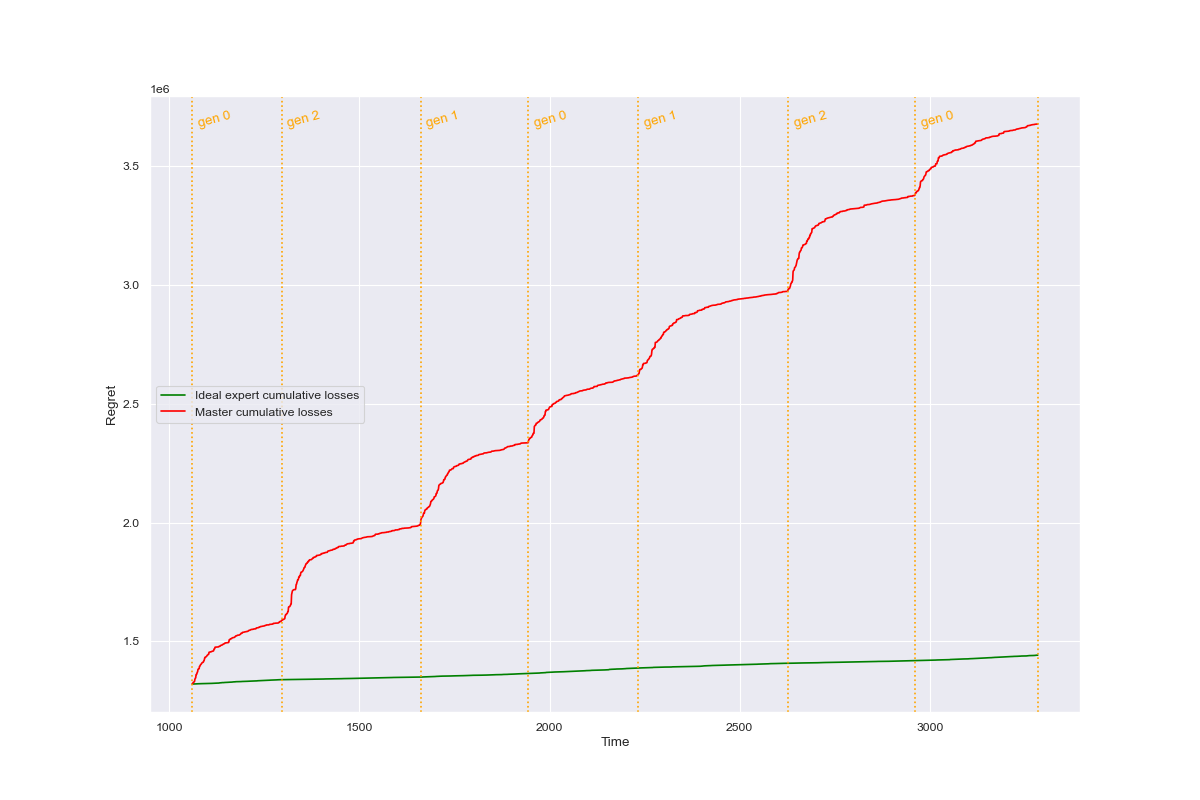
\includegraphics[width=1\linewidth]{fig}

%\begin{figure}
%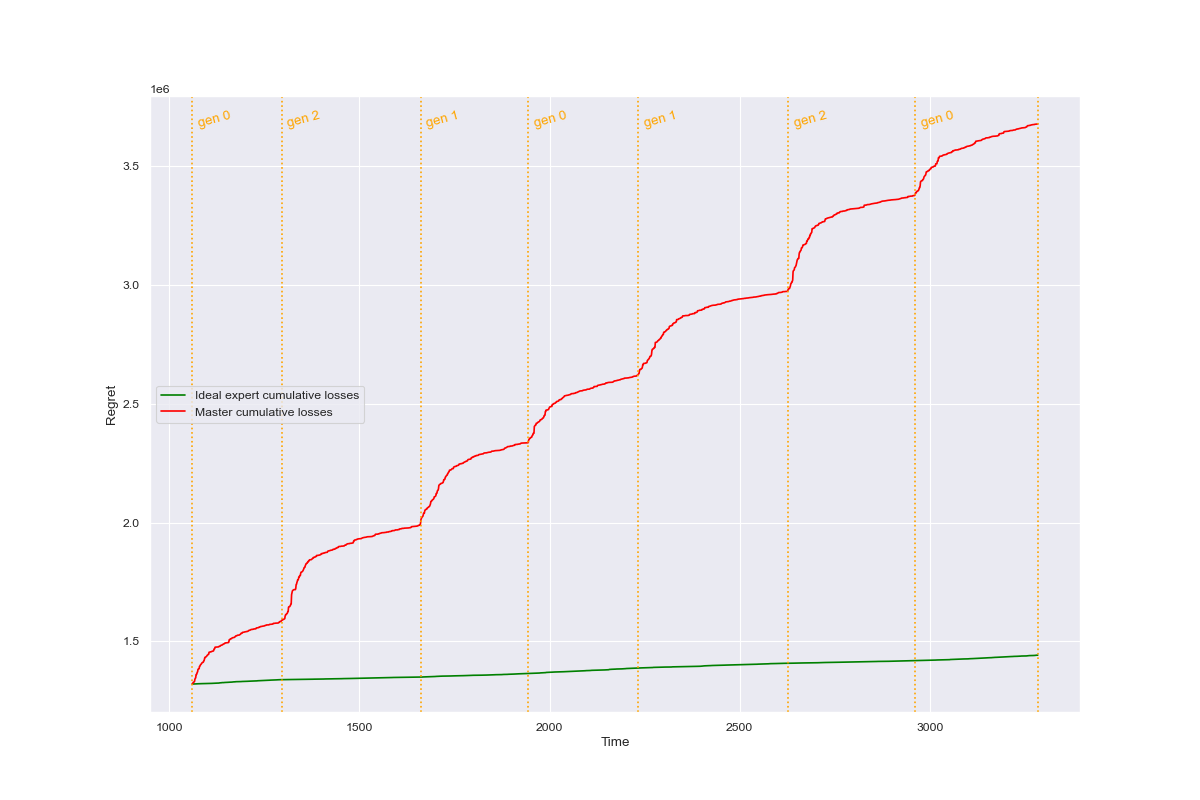
\includegraphics[width=1\linewidth]{fig}
%\end{figure}
\end{frame}

%------------------------------------------------

%\begin{frame}[fragile] % Need to use the fragile option when verbatim is used in the slide
%\frametitle{Citation}
%An example of the \verb|\cite| command to cite within the presentation:\\~
%
%This statement requires citation \cite{p1}.
%\end{frame}

%------------------------------------------------

%\begin{frame}
%\frametitle{References}
%\footnotesize{
%\begin{thebibliography}{99} % Beamer does not support BibTeX so references must be inserted manually as below
%\bibitem[Smith, 2012]{p1} John Smith (2012)
%\newblock Title of the publication
%\newblock \emph{Journal Name} 12(3), 45 -- 678.
%\end{thebibliography}
%}
%\end{frame}

%------------------------------------------------

\begin{frame}
\Huge{\centerline{The End}}
\end{frame}

%----------------------------------------------------------------------------------------

\end{document}